%%%%%%%%%%%%%%%%%%%%%%%%%%%%%%%%%%%%%%%%%%%%%%%%%%%%%%%%%%%%%%%%%%%%%%%
%% template for II2202 report
%% original 2015.11.24
%% revised  2018.08.26
%%%%%%%%%%%%%%%%%%%%%%%%%%%%%%%%%%%%%%%%%%%%%%%%%%%%%%%%%%%%%%%%%%%%%%%
%

\documentclass[12pt,twoside]{article}

\usepackage[paper=a4paper,dvips,top=1.5cm,left=1.5cm,right=1.5cm,
    foot=1cm,bottom=1.5cm]{geometry}
\usepackage[disable]{todonotes}

%\usepackage[T1]{fontenc}
%%\usepackage{pslatex}
\renewcommand{\rmdefault}{ptm} 
\usepackage{mathptmx}
\usepackage[scaled=.90]{helvet}
\usepackage{courier}
%
\usepackage{bookmark}

\usepackage{fancyhdr}
\pagestyle{fancy}

\usepackage{nameref}

\usepackage[numbers]{natbib}
\bibliographystyle{IEEEtranN}

%%----------------------------------------------------------------------------
%%   pcap2tex stuff
%%----------------------------------------------------------------------------
%  \usepackage[dvipsnames*,svgnames]{xcolor} %% For extended colors
%  \usepackage{tikz}
%  \usetikzlibrary{arrows,decorations.pathmorphing,backgrounds,fit,positioning,calc,shapes}

%% \usepackage{pgfmath}	% --math engine
%%----------------------------------------------------------------------------
%% \usepackage[latin1]{inputenc}
\usepackage[T1]{fontenc}
\usepackage[utf8]{inputenc}
\usepackage[english, romanian]{babel}
%% \usepackage{rotating}		 %% For text rotating
\usepackage{array}			 %% For table wrapping
\usepackage{graphicx}	                 %% Support for images
\usepackage{float}			 %% Suppor for more flexible floating box positioning
\usepackage{color}                       %% Support for colour 
\usepackage{mdwlist}
%% \usepackage{setspace}                 %% For fine-grained control over line spacing
%% \usepackage{listings}		 %% For source code listing
%% \usepackage{bytefield}                %% For packet drawings
\usepackage{tabularx}		         %% For simple table stretching
%%\usepackage{multirow}	                 %% Support for multirow colums in tables
\usepackage{dcolumn}	                 %% Support for decimal point alignment in tables
\usepackage{url}	                 %% Support for breaking URLs
\usepackage[perpage,para,symbol]{footmisc} %% use symbols to ``number'' footnotes and reset which symbol is used first on each page

%% \usepackage{pygmentize}           %% required to use minted -- see python-pygments - Pygments is a Syntax Highlighting Package written in Python
\usepackage{listings}		     %% For source code highlighting
\usepackage{hyperref}

\usepackage{changepage}

%% \usepackage{hyperref}		
\usepackage[all]{hypcap}	 %% Prevents an issue related to hyperref and caption linking
%% setup hyperref to use the darkblue color on links
%% \hypersetup{colorlinks,breaklinks,
%%             linkcolor=darkblue,urlcolor=darkblue,
%%             anchorcolor=darkblue,citecolor=darkblue}

%% Some definitions of used colors
\definecolor{darkblue}{rgb}{0.0,0.0,0.3} %% define a color called darkblue
\definecolor{darkred}{rgb}{0.4,0.0,0.0}
\definecolor{red}{rgb}{0.7,0.0,0.0}
\definecolor{lightgrey}{rgb}{0.8,0.8,0.8} 
\definecolor{grey}{rgb}{0.6,0.6,0.6}
\definecolor{darkgrey}{rgb}{0.4,0.4,0.4}
%% Reduce hyphenation as much as possible
\hyphenpenalty=15000 
\tolerance=1000

%% useful redefinitions to use with tables
\newcommand{\rr}{\raggedright} %% raggedright command redefinition
\newcommand{\rl}{\raggedleft} %% raggedleft command redefinition
\newcommand{\tn}{\tabularnewline} %% tabularnewline command redefinition

%% definition of new command for bytefield package
\newcommand{\colorbitbox}[3]{%
	\rlap{\bitbox{#2}{\color{#1}\rule{\width}{\height}}}%
	\bitbox{#2}{#3}}

%% command to ease switching to red color text
\newcommand{\red}{\color{red}}
%%redefinition of paragraph command to insert a breakline after it
\makeatletter
\renewcommand\paragraph{\@startsection{paragraph}{4}{\z@}%
  {-3.25ex\@plus -1ex \@minus -.2ex}%
  {1.5ex \@plus .2ex}%
  {\normalfont\normalsize\bfseries}}
\makeatother

%%redefinition of subparagraph command to insert a breakline after it
\makeatletter
\renewcommand\subparagraph{\@startsection{subparagraph}{5}{\z@}%
  {-3.25ex\@plus -1ex \@minus -.2ex}%
  {1.5ex \@plus .2ex}%
  {\normalfont\normalsize\bfseries}}
\makeatother

%% DP: making \todo[inline] actually on the same line as a paragraph
\makeatletter 
\tikzstyle{inlinenotestyle} = [
    draw=\@todonotes@currentbordercolor,
    fill=\@todonotes@currentbackgroundcolor,
    line width=0.5pt,
    inner sep = 0.8 ex,
    rounded corners=4pt]

% \renewcommand{\@todonotes@drawInlineNote}{%
%         {\begin{tikzpicture}[remember picture,baseline=(current bounding box.base)]%
%             \draw node[inlinenotestyle,font=\@todonotes@sizecommand, anchor=base,baseline]{%
%               \if@todonotes@authorgiven%
%                 {\noindent \@todonotes@sizecommand \@todonotes@author:\,\@todonotes@text}%
%               \else%
%                 {\noindent \@todonotes@sizecommand \@todonotes@text}%
%               \fi};%
%           \end{tikzpicture}}}%
% \newcommand{\mytodo}[1]{\@todo[inline]{#1}}%
\makeatother

\setcounter{tocdepth}{3}	%% 3 depth levels in TOC
\setcounter{secnumdepth}{5}

\usepackage{subcaption}

\usepackage{grffile} % To remove filename from pdf figure

\newcommand{\resnettimebfc}{$5.79\pm0.022\%$}     % ( 5.82 +  5.82 +  5.66 +  5.82 +  5.81)/5
\newcommand{\resnettimecuda}{$5.29\pm0.006\%$}    % ( 5.26 +  5.29 +  5.27 +  5.31 +  5.32)/5     9.5% slower
\newcommand{\resnettimehalloc}{$not~working$}     %
\newcommand{\alexnettimebfc}{$41.62\pm0.001\%$}   % (41.61 + 41.66 + 41.60 + 41.61 + 41.61)/5
\newcommand{\alexnettimecuda}{$40.19\pm0.002\%$}  % (40.17 + 40.26 + 40.26 + 40.06 + 40.20)/5     3.6% slower
\newcommand{\alexnettimehalloc}{$36.31\pm0.011\%$}%

%%%%%%%%%%%%%%%%%%%%%%%%%%%%%%%%%%%%%%%%%%%%%%%%%%%%%%%%%%%%%%%%%%%%
%% End of preamble
%%%%%%%%%%%%%%%%%%%%%%%%%%%%%%%%%%%%%%%%%%%%%%%%%%%%%%%%%%%%%%%%%%%%

\renewcommand{\headrulewidth}{0pt}
\lhead{II2202, Fall 2018, Period 1-2}
%% or \lhead{II2202, Fall 2016, Period 1}
\chead{Final report}
\rhead{\date{\today}}

\makeatletter
\let\ps@plain\ps@fancy 
\makeatother

\setlength{\headheight}{15pt}

%% Placed here so my diacritics ȘșȚț work. Seems to not work if above the packages or before the document begins.
% \title{GPU Dynamic Memory Allocation Algorithms for Machine Learning}
% \title{Halloc as a GPU Dynamic Memory Allocation Algorithm for Machine Learning}
%\title{Halloc as a GPU Dynamic Memory Allocation Algorithm for TensorFlow}
%\title{Halloc as a GPU Dynamic Memory Allocation Algorithm for Machine Learning with TensorFlow}
\title{Dynamic memory allocation on the GPU for Machine Learning: Improving performance of TensorFlow with Halloc}
\author{
        \textsc{Erik H. Wouters}
            \qquad
        \textsc{Dragoș Ș. Perju} % ȘșȚț -- These are not in the "standard cedilla" romanian keyboard, just "standard" romanian keyboard
        \mbox{}\\
        \normalsize
            \texttt{ehwo}
        \textbar{}
            \texttt{dsperju}
        \normalsize
            \texttt{@kth.se}
}
\date{\today}


\begin{document}

\selectlanguage{english}

\maketitle

\begin{abstract}
\label{sec:abstract}

This paper compares three dynamic memory allocators designed for running on GPUs and select the best performing allocator for TensorFlow’s Convolutional Neural Network (CNN) benchmark, running the ResNet-50 and AlexNet models. Allocators that are considered are \texttt{BFCMalloc}, \texttt{CUDAMalloc} and \texttt{Halloc}. The The main metric of comparison is the number of images per second processed by the benchmark. Other metrics studied are: object sizes requested for allocation and the impact of several parameters of \texttt{Halloc} on the speed of the benchmark. Previous research shows that \texttt{Halloc} performs well on workloads with many small allocations, whereas \texttt{CUDAMalloc} performs slower for the same workload\cite{Vinkler2015}. We show that ResNet-50 and AlexNet do have this type of workload. Our implementation of \texttt{Halloc} is $13\%$ slower than \texttt{BFCMalloc} due to inefficent use of the CUDA library, which causes unnecessary overhead. We also provide a statistical model that shows that the occupancy fraction at which a slab is considered roomy (\texttt{ROOMY\_FRACTION}) has a significant impact on the speed of the benchmark.


\textbf{Keywords:} Algorithm, Performance, Machine learning, GPU, Dynamic memory, Allocation, TensorFlow

\end{abstract}
%%\clearpage

\selectlanguage{english}
\tableofcontents

\section*{List of Acronyms and Abbreviations}
\label{list-of-acronyms-and-abbreviations}

\begin{basedescript}{\desclabelstyle{\pushlabel}\desclabelwidth{10em}}
\item[CNN]					Convolutional Neural Network
\item[CPU]                  Central Processing Unit
\item[CUDA]                 Compute Unified Device Architecture
\item[GPU]                  Graphics Processing Unit
\item[ML]                   Machine Learning
\item[SIMD]                 Single-Instruction Multiple-Data
\end{basedescript}


% \clearpage

\section{Introduction}
\label{sec:introduction}
%% Longer problem statement
%% General introduction to the area

\citeauthor{mach-learning-matters} (\citeyear{mach-learning-matters}) \cite{mach-learning-matters} says that "much of machine learning research is inspired by weighty problems", such research trying to solve issues from biology, medicine, finance, astronomy, agriculture etc. Indeed, machine learning is one of the technologies which succeeds to influence the real-world in a major way, helping with concrete issues such as: water pipe risk assessments \cite{water-pipe-risk}, detecting aviation turbulence \cite{aviation-turbulence}, medicine/drug discovery \cite{drug-discovery} and so on. It is therefore important to work on achieving better performances of the underlying processes that stand behind such a complex technology, with such a big impact on our society. Machine learning (ML) is empowering smartphones \cite{google-visual-core} and IoT devices \cite{visual-core-iot} today, as well, meaning improving the performances of ML algorithms can also lower power consumption of such devices.

We aim to improve machine learning by touching one of the basic computing techniques it uses: the dynamic memory allocation that happens on the graphics processing unit (GPU). 

In the present work, we consider \texttt{Halloc} \cite{halloc-paper} to replace \texttt{CUDAMalloc} and \texttt{BFCAlloc} that are currently the only options for use for TensorFlow - a well-known software library for machine learning \cite{TensorFlow-main-paper}. TensorFlow offers \texttt{CUDAMalloc} and \texttt{BFCAlloc} as algorithms for use when allocating memory dynamically on the GPU, needed for working with machine learning structures - such as Convolutional Neural Networks (CNNs). We choose to experiment using TensorFlow, as it is a popular software platform for machine learning, being involved in a large number of real-world applications \cite{drug-discovery} \cite{brain-tumor-detection} \cite{security-system}. 

We consider \texttt{Halloc} after a thorough search of GPU dynamic memory allocators that are publicly available today. We describe in the paper why we chose \texttt{Halloc} as our main algorithm for the study. We compile a TensorFlow version that integrates \texttt{Halloc} as its main choice for GPU dynamic memory allocation and run the recommended benchmark program by the TensorFlow team, using the metric "images per second" to study wanted performance changes.

TensorFlow, its benchmark, AlexNet (the CNN model ran by the benchmark) and \texttt{Halloc} are all described under the sub-section \textit{\ref{sec:theoretical-framework} \nameref{sec:theoretical-framework}} of this \textit{\nameref{sec:introduction}} section. In section \ref{sec:questions}, \textit{\nameref{sec:questions}}, it is laid out the concrete goals of this study, as well as some predictions we can make. Section \ref{sec:methods}, \textit{\nameref{sec:methods}}, includes the system setup on which the the tests were executed, as well as the description of the test paradigm this study entails. Section \ref{sec:results-and-analysis}, \textit{\nameref{sec:results-and-analysis}}, includes the final graphs and tables with data after an extensive run of our tests. Finally, under the section \ref{sec:discussion}, \textit{\nameref{sec:discussion}}, we draw a conclusion of the impact we observe when using TensorFlow with \texttt{Halloc}. 

\section{Theoretical framework}
\label{sec:theoretical-framework}

\subsubsection*{Literature study}

Publications studying comparisons specifically, of different GPU dynamic memory allocators, are scarce in today's literature. Dynamic memory allocation for GPU in its whole is not a subject that is well sought after. Only the few algorithms themselves that do exist have, in their documentation, also comparisons with the previous algorithms, for evaluations purposes. Such a list of algorithms is described later in this section, along with \texttt{Halloc}, our main choice.

A thorough comparison that is indeed in literature, however, is the work of \citeauthor{Vinkler2015} from \citeyear{Vinkler2015}, which has, as its main purpose, to do a comprehensive comparison of many GPU dynamic memory allocation algorithms under the premise of running a workload of \textit{k}-d tree data structures. Such structures are mainly used in ray tracing, to produce lighting and shadows when rendering 3D images. \citeauthor{Vinkler2015} (\citeyear{Vinkler2015}) select many dynamic memory allocators and integrate them into their own benchmark, as well as create their own, new dynamic memory allocator specific for their workflow, namely the \texttt{CMalloc}. All of this is packaged in a source code provided freely to the public. We use their source code as a start to our own implementation.

\subsubsection*{TensorFlow \& the default allocators}

TensorFlow is an open-source software library with a focus on building neural network architectures, and then training and applying the models \cite{TensorFlow-main-paper}. It performs machine learning in a fast and easy manner, being one of its main application purposes. TensorFlow was developed and used in-house by a research team at Google, being released afterwards to the public on November 2015 on GitHub. The very first public version of TensorFlow contains parts of another deep learning project named Caffe, developed at University of California, having a copyright notice alongside, dated 2014.

Yet, ever since TensorFlow was developed, its main dynamic memory allocation algorithm for GPU use is the \texttt{BFCAllocator}. In its own source code, \texttt{BFCAllocator} is described to be: "\textit{a memory allocator that implements a 'best-fit with coalescing' algorithm.  [...] [It] is essentially a very simple version of Doug Lea's malloc (dlmalloc)" \cite{Vinkler2015}}. Doug Lea's allocation algorithm is generally used for CPU applications and described in a later subsection. 

CUDA's own dynamic memory allocator, \texttt{CUDAMalloc}, is kept as a selectable alternative to use with TensorFlow. It is however a proprietary algorithm and, therefore, there is no code shared for study but the header file that exposes the functions' declarations for use. However, after performance measurements, \citeauthor{Vinkler2015} (\citeyear{Vinkler2015}) states that \texttt{CUDAMalloc} is relatively slow for allocations of small sized objects \cite{Vinkler2015}, an aspect that can be important for the pattern of objects TensorFlow allocates.

\subsubsection*{Dynamic memory allocation}

Dynamic memory allocation is a technique well-known and often used by programmers. Much of the work for improvement and research on this topic is being devoted to the context of single-core and multi-core general purpose processors \cite{YOU2015}. Comparing to static memory allocation, which happens at program compilation time and is more frequently used in programming, dynamic memory allocation brings along issues with its use, such as fragmentation and memory leaks \cite{TRAISTER199099}.

Such problems make dynamic memory allocation algorithms unsuitable for use on specific platforms, such as safety-critical embedded systems \cite{Puaut_2002}. The technique however did progress to be implemented on other hardware than CPUs. GPUs introduce new difficulties in implementing dynamic memory allocation, being many-core systems running many more threads, distributed on many more cores than general purpose processors can have. GPUs however evolved to be used for more than just rendering images, being used for complex programming techniques such as machine learning. 

Machine learning takes advantage of GPUs \cite{deep-learning-gpu}, using their multiple core setup, threading capabilities and single-instruction multiple-data (SIMD) type of computation in order to achieve more-than-average performance than running on general purpose processors. This makes GPU dynamic memory allocation important in the context of such applications.


\subsubsection*{Selected allocators}

In this section, we discuss \texttt{BFCMalloc} and \texttt{CUDAMalloc}, the two allocators already integrated in TensorFlow, together with our allocator of choice, \texttt{Halloc}, to be integrated in the TensorFlow code and in our tests.

\textbf{BFCMalloc:} As mentioned, \texttt{BFCMalloc} is a best-fit with coalescing allocator, inspired from Doug Lea's malloc. Doug Lea's malloc \cite{dlmalloc} is a CPU dynamic memory allocation algorithm, that keeps ordered bins of different sizes (linked lists of addresses of free memory chunks), starting from as small as 16 bytes for 32-bit systems or 24 bytes for 64-bit systems and incrementing by 8 bytes up to 512 bytes, after which the sizes kept are approximately logarithmic in size up to the capacity allowed, needing to be 128 fixed-size bins in total (including the bins below 512 bytes). As memory of a specific size is requested, Doug Lea's malloc searches from the smallest to the largest bin, by size, for the first available chunk address that is unoccupied. This algorithm has not been compared with others in literature, being specific to TensorFlow.

\textbf{CUDAMalloc:} \texttt{CUDAMalloc} is a proprietary algorithm from NVIDIA. Its internal workings are not documented, however the algorithm is fairy used in comparisons as a baseline. It is therefore obviously noted as the slowest, other algorithms being developed trying to surpass it in its performances \cite{halloc-paper} \cite{Vinkler2015}.

\textbf{Halloc \cite{halloc-paper}:} \texttt{Halloc} separates the available memory into two parts and manages only one part, for objects of size under 3 kilobytes, while the other it leaves for use with \texttt{CUDAMalloc} for larger sized allocations. The part of memory it manages is separated in slabs, of which status (free/occupied) is saved in a bitmap. The bitmap is searched using a hashing function for speed. A "slab" is a group of chunks of equal size, and different slabs can have different chunks. Slabs are assigned during runtime to different sizes and can get re-assigned if they become free, also during runtime. \cite{Vinkler2015}. \texttt{Halloc} implements atomic functions, that it uses to quickly to mark and unmark the bitmap at once -- actions that can be done by any thread on the GPU that wants to allocate memory. By using the hashing function for searching, it avoids the situation when two threads pick and search the same part of the bitmap, meaning the atomic functions would clash \cite{Vinkler2015} and queue for sequential instead of parallel execution. \texttt{Halloc} reports to have between 3 to 1000 times better performances than \texttt{ScatterAlloc}, depending on the number of threads allocating at the same time \cite{halloc-paper}.

\textbf{Other allocators:} More allocators have been developed for the GPU, the ones that had the potential to replace \texttt{Halloc} in this research being \texttt{XMalloc} \cite{xmalloc}, \texttt{ScatterAlloc} \cite{scatter-alloc}, \texttt{FDGMalloc} \cite{fdgmalloc} and \texttt{CMalloc} \cite{Vinkler2015}.

\begin{itemize}

\item \texttt{XMalloc} is faster by 2.5 to 10 times than \texttt{CUDAMalloc} in \texttt{ScatterAlloc}'s tests \cite{scatter-alloc};

\item \texttt{ScatterAlloc} is faster by 10 to 100 times than \texttt{CUDAMalloc} is its own tests \cite{scatter-alloc};

\item \texttt{FDGMalloc} is faster by 5 to 50 times than \texttt{ScatterAlloc} in its own tests \cite{fdgmalloc} (the same tests also show \texttt{ScatterAlloc} is 60 times slower than \texttt{CUDAMalloc} in most parts, but not faster than \texttt{FDGMalloc});

\item \texttt{CMalloc}, while the result of \citeauthor{Vinkler2015} (\citeyear{Vinkler2015}) \cite{Vinkler2015} after a study and comparison of all of the algorithms above, it is an algorithm that tries not to favour smaller allocations over bigger ones in speed, which is what we desire when working with TensorFlow (as stated also in the next section, \textit{\nameref{sec:questions}}).

\end{itemize}

Our study therefore proceeds by using \texttt{Halloc} as the designated allocator for replacement over the standard used by TensorFlow. Literature holds the fact that it is faster than all of the alternatives found, for smaller object sizes that we suspect TensorFlow will often request.

% Literature:
% \url{https://devtalk.nvidia.com/default/topic/878664/custom-memory-allocator-for-cuda-desired/}
% \url{https://riptutorial.com/TensorFlow/example/13427/use-the-tcmalloc-allocator}
% \url{http://on-demand.gputechconf.com/gtc/2014/presentations/S4271-halloc-high-throughput-dynamic-memory-allocator.pdf}

%Different programming languages offer different ways of managing variables. Most of them use a dynamic memory allocation algorithm. This algorithm returns a memory address when request to create a new variable is executed. In higher level programming languages there is no direct interaction with the memory addresses, but in lower level languages programmers can employ advanced techniques to manage the memory more efficiently for a specific application \cite{TRAISTER199099}.

\section{Research questions}
\label{sec:questions}

In this section we discuss the hypothesis that we are attempting to judge in the current study.

TensorFlow already implements \texttt{CUDAMalloc} and \texttt{BFCMalloc} as its two selectable options for GPU method of allocation, with the latter being the default. We were therefore able to do an initial run of the benchmark. In our initial comparison, \texttt{CUDAMalloc} achieves \resnettimecuda\ images per second performance when running the ResNet-50 benchmark, while \texttt{BFCMalloc} attains \resnettimebfc\ images per second, showing that, in fact, dynamic memory allocation algorithms can have an impact on the overall performance of machine learning software.

Our main metric for comparison is, indeed, the speed of training of the neural network model (ResNet-50, AlexNet) that the benchmark can attain, expressed in images per second. It is the main output that the benchmark shows while executing. We want to attain a bigger performance than the default allocators, after our modification. 

We are suspecting that TensorFlow will be allocating most of its objects in small sizes. As such, we study the object sizes that are being allocated throughout the runtime of the benchmark in order to justify selecting an allocator that favours smaller allocations in speed, over bigger sized objects. 

The allocator chosen for the study, \texttt{Halloc}, has a number of parameters available for configuration -- that might yield different results for the study of performance. We therefore study if such parameters influence the yield of the benchmark.

As a summary, the hypothesis we are trying to approve or deny are listed below:



% \textbf{\textit{Maybe this book can be cited somewhere:}} \cite{GINSBURG2017345} \\

% CUDA offers, to programmers who want to take advantage of GPU's processing power, a proprietary, unpublished algorithm for dynamically allocating memory called \texttt{CudaMalloc}. However, dynamic memory allocation algorithms running on the CPU are often customized for certain programs that require the edge in speed or stability, such as video games, database engines and so on. It is only natural to suspect that Machine Learning algorithms would be able to deliver faster performances if an allocator tailored for their needs would be selected as well.

% We believe that \texttt{CudaMalloc}, as a general purpose dynamic memory allocation algorithm for the GPU, can be replaced for better performances when using the TensorFlow \cite{abadi2016} library for Machine Learning processing. In particular the ResNet-50 implementation of TensorFlow will be evaluated, which is a Convolutional Neural Network (CNN) with many layers and will therefore allocate many small sized objects in the GPU memory \cite{DBLP:HeZRS15}.
% Algorithms that possibly perform better are mentioned in the work of \citeauthor{Vinkler2015} \cite{Vinkler2015}. They state that \texttt{CudaMalloc} is slower to process than other allocation algorithms for allocating many small sized objects, as shown in Figure 3a in \cite{Vinkler2015}. We decide to therefore select the better allocation algorithm for the task at hand, through the proposed research.

\begin{enumerate}
\item Using \texttt{Halloc} with TensorFlow, which is described to be much faster than \texttt{CUDAMalloc} (3 to 3000 times) [2], will bring a performance improvement to the speed of TensorFlow's benchmark (images per second);
\item TensorFlow allocates many smaller-sized objects, for which \texttt{Halloc} can be beneficial as it favours in speed though its design;
\item The configurable parameters of \texttt{Halloc} do not influence the speed of the benchmark. (Through denying this hypothesis, we manage to correlate the performance with \texttt{Halloc}'s parameters)
\end{enumerate}


% \subsubsection{Problem Statement}
% \label{sec:problem-statement}

%\todo{Describe the problem(s) that have been found in the area described in the background. Describe the problem area (in detail). For example:}

% \subsection{Problem}
% \label{sec:problem}

%\todo{State a clear and concise problem that is going to be investigated.  Answer the question What is the real problem? - What is the problem or value proposition addressed by the project? – Ideally one sentence that is very concrete. For example:}

%Fast Machine Learning processing imposes specific constraints of the dynamic memory allocator that runs on the GPU, 

% The memory allocation pattern of TensorFlow's implementation of ResNet-50 is not a great match for the memory allocator TensorFlow uses, we will investigate which previously published dynamic memory allocation algorithms perform better.

%The need for fast Machine Learning processing, by improving the dynamic memory allocation that runs on the GPU.

%Select the fastest, state of the art, open source GPU dynamic memory allocation algorithm for a Machine Learning workload.

% \subsection{Hypothesis}
% \label{sec:hypothesis}

%\todo{State a hypothesis that you think would be the outcome of your investigation. Answer the question: What is your hypothesis? (Note that the hypothesis must be measurable to be confirmed or falsified. Moreover not all projects have hypothesis.).}

% Our hypothesis is that one or more of the algorithms described by \citeauthor{Vinkler2015} \cite{Vinkler2015} perform better as a memory allocator for TensorFlow's implementation of ResNet-50 than the stock \texttt{BFCAllocator} or the standard \texttt{CudaMalloc} does, in terms of overall speed, fragmentation and stability.

%when allocation requests vary in size or frequency (consecutive or varied requests).

% \subsection{Purpose}
% \label{sec:purpose}

%\todo{Explain the purpose(s) of your project / investigation (the expected deliverables from the project). Answer the question: Why do this project? (purpose/effect, i.e. – the purpose can be to save environment but the goal is to build a robot that can pick up trash.) Why would you carry out the project? For example:}

% Machine Learning is a technology that helps with the advancement on many problems we are struggling with today. From drug discovery \cite{Ramsundar_Kearnes_Riley_Webster_Konerding_Pande_2015} to sorting cucumbers by quality \cite{cucumber}, Machine Learning has applications in domains such as medical, agricultural, security, marketing and many others. It is through the presented project that we want to contribute to the progress of a programming tool that betters the lives of people.

% \subsection{Goal(s)}
% \label{sec:goal(s)}

%\todo{Explain the goal(s), objective(s), and/or the result(s) of your investigation. What are the expected deliverables/outcomes from the project? For example:}

% 1. Design a repeatable experiment that shows that one of the GPU memory allocation algorithms presented by \citeauthor{Vinkler2015} \cite{Vinkler2015} is faster than the standard \texttt{CudaMalloc} function. This experiment will be used to validate the hypothesis. 2. Understand why this algorithm is faster (or slower).
% If we find a faster algorithm, send results and recommendation to the TensorFlow team for study and possible implementation in the release version.


\section{Methods}
\label{sec:methods}

%\todo{Describe and explain the research methods that will be used for the project. What research method (or methods) will be used? Argue: why this is the most appropriate method or methods. For example:}

Our methodology is as follows:
\begin{enumerate}
    \vspace{-3px}
    \itemsep-0.25em
    \item Analyze memory allocation pattern of ResNet-50, AlexNet;
    \item Match pattern to memory allocator suggested by literature (\texttt{Halloc});
    \item Add \texttt{Halloc} allocator to TensorFlow source code;
    \item Use standard benchmarks on modified TensorFlow, to evaluate the performance compared to the built-in memory allocators;
    \item \texttt{Halloc} is configurable through different parameters -- evaluate performance by changing them systematically.
\vspace{-3px}
\end{enumerate}

Manual modifications of TensorFlow's source code, to introduce small snippets that collect data, were used to gain insight in the memory allocation pattern of ResNet-50. We then studied the literature to find GPU memory allocation algorithms that were likely to perform well on this specific memory allocation pattern. From this literature study the \texttt{Halloc} algorithm was the most promising. We located the appropriate sections of code in the huge code base of TensorFlow and integrated the open source \texttt{Halloc} implementation\footnote{Available at \url{https://github.com/canonizer/halloc}\\}.

% - Argue that memory map is quite unuseful

% -  we inject the code to provide output information of the sizes of objectes requested for allocation by the benchmark. In such a way, we know w

% Focusing on such a metric means we maintain the 

\todo[inline]{Also, we deem of interest to try out different model sizes, in order to see not only the speed of certain allocation algorithms, but how well they manage the memory throughout the benchmark run, possibly running slower in general but are able to construct a bigger model fully than its counterparts, which can interrupt unwantingly mid-way.}


\subsubsection*{Benchmarking Methods}

The edited TensorFlow code\footnote{Available at \url{https://github.com/dragosprju/TensorFlow/tree/halloc}\\} was compiled on a HP ZBook 15 workstation laptop, equipped with an NVIDIA K1100M GPU. Then, TensorFlow's Convolutional Neural Network benchmarks\footnote{Available at \url{https://github.com/TensorFlow/benchmarks}\\} were run. As these benchmarks are well known in the Machine Learning field, this provides results that mimic real world performance of these algorithms applied to Machine Learning \cite{abadi2016}. 

The full benchmark, as it is from the TensorFlow's website, could not run on the NVIDIA K1100M GPU, being out of memory. Decreasing the batch size from 32 to 16 fixed this problem. In order to create results that are as repeatable as possible, each test was run 5 times and then the times were averaged together. The NVIDIA K1100M GPU ran in it's default state. For each run of the benchmarks, ten warm-up steps were performed and the next 100 steps were averaged.

%The project uses the empirical method \cite{bock2001}. 

\vspace{10px}

Replication information:
\begin{itemize}
\vspace{-5px}
\itemsep-0.25em 
    \item Bazel 0.18.1
    \item CUDA 9.0
    \item cuDNN 7.0.5 %(we must mention 7.0.5 vs 7.4 is 3 times slow %\url{https://developer.nvidia.com/sites/default/files/akamai/deeplearning/cudnn/cudnn_7.4_cnn_1.png})
    \item gcc 6.4.0 (symlinked to /usr/bin/gcc)
    \item Ubuntu 18.04 LTS (Linux kernel 4.15.0-39-generic)
    \item TensorFlow v1.11.0
    \item Python 3.5.6 Anaconda
    \item Halloc 0.11\footnote{Available at \url{https://github.com/canonizer/halloc}\\}
% \vspace{-10px}
\end{itemize}

TensorFlow needs specific configuration prior to its compilation. The \texttt{configure} script of TensorFlow's source code displays self-explanatory prompts that the user must manually respond to. As TensorFlow's re-configuration and re-compilation was frequently needed for this study, a bash script was created to simplify the process of this. The script is listed in Appendix \ref{apx:bash-script} for replication purposes, which includes the re-installation command and execution of TensorFlow's benchmark\footnote{Available at \url{https://github.com/TensorFlow/benchmarks}\\}.

%\textbf{Notes about Bazel}

\subsubsection*{Parameter Sweep}
%\textbf{Write about how we tried many Halloc configurations, describe them}
\citeauthor{Vinkler2015} (\citeyear{Vinkler2015}) describe in \cite{Vinkler2015} that the \texttt{Halloc} algorithm performs well for workloads that allocate many small variables. The \texttt{Halloc} algorithm has many parameters that can be tuned to match a specific workload. In order to test the influence of such parameters on the performance, a parameter sweep was performed on the them. Only a single parameter was changed from the default at a time. The following parameter have been considered in the parameter sweep:
\begin{itemize}
\vspace{-3px}
\itemsep-0.25em 
\item \texttt{HALLOC\_FRACTION}: Memory fraction available to \texttt{Halloc} allocator, the rest goes to CUDA for
	larger allocations.
\item \texttt{BUSY\_FRACTION}: Occupancy fraction at which a slab is considered busy.
\item \texttt{ROOMY\_FRACTION}: Occupancy fraction at which a slab is considered roomy.
\item \texttt{SPARSE\_FRACTION}: Occupancy fraction at which a slab is considered sparse.
\item \texttt{MAX\_BLOCK\_SZ}: Allocations larger than this number in bytes go to CUDA for allocation. (Default: 3 kB)
\item \texttt{MAX\_NSIZES}: Maximum number of sizes supported.
\item \texttt{MAX\_NCHUNK\_IDS}: Maximum number of different chunk sizes supported.
\item \texttt{BLOCK\_STEP}: Block step (16 bytes by default), a power of two.
\item \texttt{MIN\_BLOCK\_SZ}: Minimum block size, allocations smaller than this will be allocated to this size.
% \vspace{-10px}
\end{itemize}

A linear model was fit to the data to evaluate their influence on the speed of the benchmark\footnote{Available from \texttt{\href{https://github.com/EWouters/II2202-Research-Methodology-and-Scientific-Writing---Report/blob/master/Quantitative_Python/Parse2csv.ipynb}{https://github.com/EWouters/II2202-Research-Methodology-and-Scientific-\\Writing---Report/blob/master/Quantitative\_Python/Parse2csv.ipynb}}\\}. This model was used to test the hypothesis that each of the parameters does not influence the speed of the benchmark.

This method was only used to evaluate the performance of \texttt{Halloc} on AlexNet because ResNet-50 expects aligned memory and was therefore incompatible with the \texttt{Halloc} implementation.

\subsubsection*{Time \& other considerations}

The ResNet-50 benchmark in its standard form (with batch size $16$) took about $5.5$ minutes to run. The full benchmark runs $110$ iterations including the warm-up. To analyze only a single iteration using the runtime CUDA debugging platform from NVIDIA -- the NVIDIA Visual Profiler -- takes $17$ hours. It was therefore not feasible to run the full benchmark (with $110$ iterations) with the NVIDIA Visual Profiler. We have therefore used manual code modifications to obtain data (such as that of memory allocation pattern).

Initial tests showed that profiling GPU accelerated sessions in TensorFlow took a lot of compute time. Compiling TensorFlow took about two hours on the workstation that is used for benchmarking. The compilation had been repeated a few hundred times. This amounts to a lot of time spent to generate the results. Using a GPU cluster and a compile cluster would have drastically sped up the research.

It is relevant to state that this field is rapidly developing. There are many versions of software packages available and the combinations of all these versions may have an impact on the performance. Since we have frozen the versions of the software we use three of the packages have released new versions. The biggest version issue we experienced is related to the GPUs compute capability, which is lower than recommended by TensorFlow.

\section{Results and Analysis}
\label{sec:results-and-analysis}

\subsubsection*{Memory Allocation Pattern}
Profiling a single iteration of TensorFlow's benchmark provided enough insight in the memory allocation pattern for matching with a dynamic allocation algorithm from the literature study. In order to measure the memory allocation pattern of a complete run of the benchmark, we modified the source code of TensorFlow to write all the sizes of the allocations to a file. The results of the memory allocation analysis can be found in figure \ref{fig:hist}. This figure shows that in both models small objects get allocated over an order of magnitude more often than big objects. The effect is strongest for ResNet-50. For ResNet-50 $19\%$ of the allocations are $16$ bytes or smaller while for AlexNet that fraction is $14\%$. The percentage of allocations that would be handled by \texttt{Halloc} is $48\%$ for ResNet-50 and $30\%$ for AlexNet.

\begin{figure}[!ht]
  \centering
  \begin{subfigure}[b]{0.49\textwidth}
    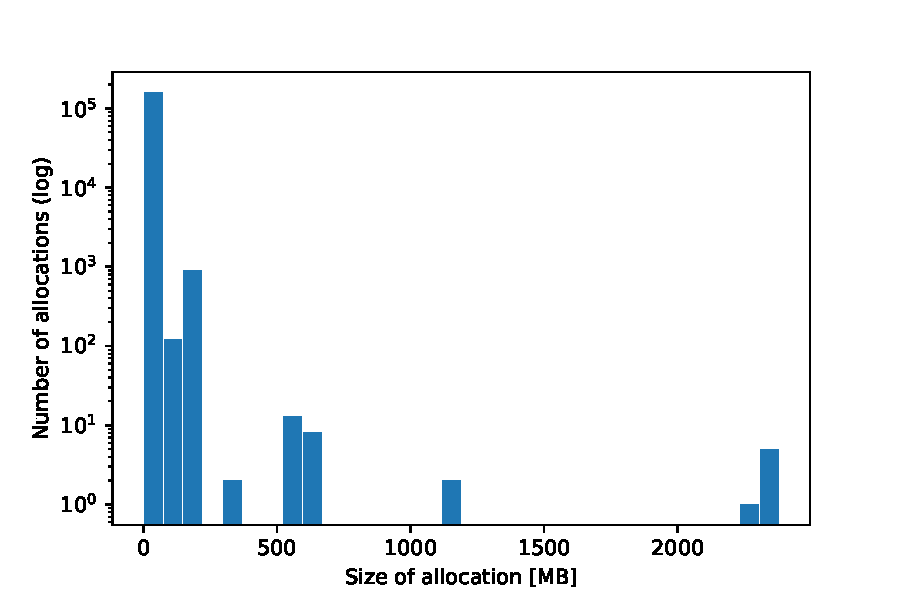
\includegraphics[width=\textwidth]{../Quantitative_Python/ResNet-50_hist_MB_ylog.pdf}
    \caption{ResNet-50}
  \end{subfigure}
  \begin{subfigure}[b]{0.49\textwidth}
    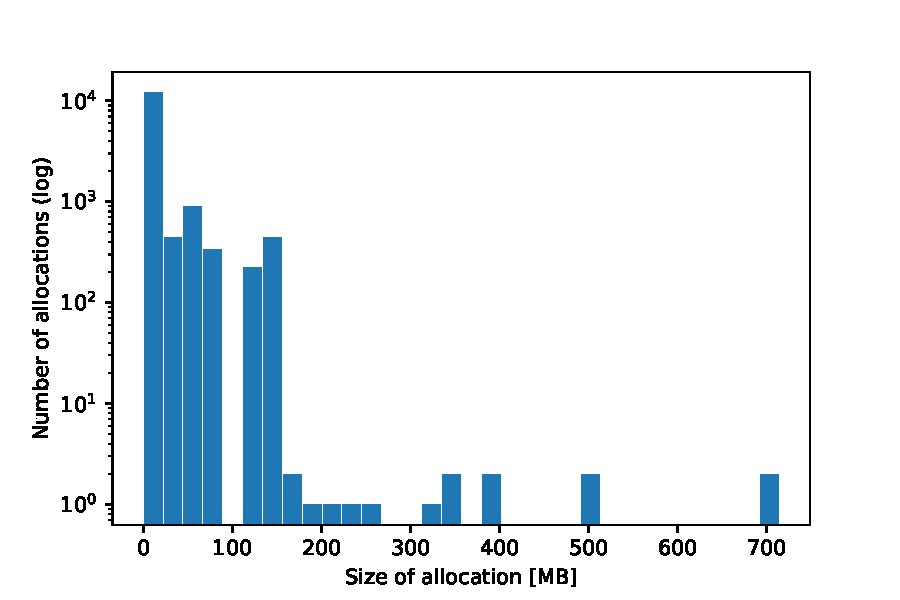
\includegraphics[width=\textwidth]{../Quantitative_Python/AlexNet_hist_MB_ylog.pdf}
    \caption{AlexNet}
  \end{subfigure}
  \caption{Histogram of object sizes requested for allocation for the two models ($32$ bins). Note that the number of allocations is depicted on a logarithmic scale, so each division is an order of magnitude.}
  \label{fig:hist}
\end{figure}

\subsubsection*{Benchmarks}
In our comparisons, we have found TensorFlow's default allocator, \texttt{BFCAllocator}, to attain \resnettimebfc\ images per second when processing the ResNet-50 model benchmark, while \texttt{CUDAMalloc} attains only \resnettimecuda\ images per second. This proves that there is significance in such a research, as choosing the right dynamic memory allocator can have a large impact on the performance of high end algorithms and computing techniques.

The benchmarks are shown in table \ref{tab:results}. The "images/sec" column shows the average amount of images that are processed per second for the different models and allocators.

\begin{table}[!ht]
\centering
\caption{Benchmark Results}
\label{tab:results}
\begin{tabular}{|l|l|l|l|}
\hline
\textbf{Model}     & \textbf{Batch size}  & \textbf{Allocator}          & \textbf{Images/sec}         \\ \hline
ResNet-50 & $16$        & \texttt{BFCMalloc} & \resnettimebfc     \\ \cline{3-4} 
          &             & \texttt{CUDAMalloc}  & \resnettimecuda    \\ \cline{3-4} 
          &             & \texttt{Halloc}    & \resnettimehalloc  \\ \hline
AlexNet   & $32$        & \texttt{BFCMalloc} & \alexnettimebfc    \\ \cline{3-4} 
          &             & \texttt{CUDAMalloc}  & \alexnettimecuda   \\ \cline{3-4} 
          &             & \texttt{Halloc}    & \alexnettimehalloc \\ \hline
\end{tabular}
\end{table}

\subsubsection*{Parameter Sweep}
The results of the parameter sweep for \texttt{Halloc} on AlexNet can be seen in table \ref{tab:parametersweep}. Except for the intercept and the \texttt{ROOMY\_FRACTION}, none of the parameters are statistically strong enough to proof that they have an effect on the speed of the benchmark. The \texttt{ROOMY\_FRACTION} has a p-score of $0.01$, from which we can reject the hypothesis that the \texttt{ROOMY\_FRACTION} does not have an effect on the speed of the benchmark.

It was expected that there would be a larger effect as $30\%$ of the allocations used \texttt{Halloc} instead of \texttt{CudaMalloc}. Unfortunately ResNet-50 could not be tested, but for that model $48\%$ of the allocations would be handled by \texttt{Halloc}. This leads us to the conclusion that even though there is a large number of small allocations, this does not make up a large portion of the total compute time of the benchmark.


\begin{table}[!ht]
\caption{Results of parameter sweep for \texttt{Halloc} on AlexNet. The default column shows the default value. The Min and Max columns show the boundaries of the parameter sweep. The step column shows the step size in case of linear steps, and $2^x$ if exponential steps are used ($x$ increases in steps of $1$ from Min to Max). The four rightmost columns show a linear model fit to the data.}
\label{tab:parametersweep}
\begin{adjustwidth}{-0.55cm}{}
\begin{tabular}{|l|l|l|l|l|l|l|l|l|}
\hline
\textbf{Parameter}        & \textbf{Default} & \textbf{Min}  & \textbf{Max}  & \textbf{Steps}         & \textbf{Coefficient} & \textbf{Standard error} & \textbf{t-score} & \textbf{p-score} \\ \hline
Intercept                 &           &        &        &         & $36.6428$     & $2.561$          & $14.306$  & $0.000$   \\ \hline
\texttt{HALLOC\_FRACTION} & $0.25$    & $0.00$ & $1.00$ & $0.10$  & $0.3146$      & $0.389$          & $0.808$   & $0.422$   \\ \hline
\texttt{BUSY\_FRACTION}   & $0.835$   & $0.70$ & $0.90$ & $0.05$  & $-4.2388$     & $2.840$          & $-1.493$  & $0.141$   \\ \hline
\texttt{ROOMY\_FRACTION}  & $0.60$    & $0.50$ & $0.80$ & $0.05$  & $4.5185$      & $1.702$          & $2.654$   & $0.010$   \\ \hline
\texttt{SPARSE\_FRACTION} & $0.012$   & $0.02$ & $0.20$ & $0.02$  & $1.5030$      & $1.501$          & $1.001$   & $0.321$   \\ \hline
\texttt{MAX\_BLOCK\_SZ}   & $3072$    & $4$    & $12$   & $2^x$   & $-6.755e-05$  & $6.59e-05$       & $-1.026$  & $0.309$   \\ \hline
\texttt{MAX\_NSIZES}      & $16$      & $0$    & $8$    & $2^x$   & $0.0015$      & $0.002$          & $0.782$   & $0.437$   \\ \hline
\texttt{MAX\_NCHUNK\_IDS} & $8$       & $0$    & $6$    & $2^x$   & $0.0076$      & $0.008$          & $0.940$   & $0.351$   \\ \hline
\texttt{BLOCK\_STEP}      & $16$      & $0$    & $7$    & $2^x$   & $0.0016$      & $0.004$          & $0.403$   & $0.688$   \\ \hline
\texttt{MIN\_BLOCK\_SZ}   & $16$      & $0$    & $8$    & $2^x$   & $0.0021$      & $0.002$          & $1.115$   & $0.269$   \\ \hline
\end{tabular}
\end{adjustwidth}
\end{table}


\section{Discussion}
\label{sec:discussion}

In the current study, we attempt to improve TensorFlow's performance through changing its dynamic memory allocation algorithms that come by default. For this, we find a new allocator for replacement by first studying the documentation of different algorithms that are available publicly: \texttt{XMalloc} \cite{xmalloc}, \texttt{ScatterAlloc} \cite{scatter-alloc}, \texttt{FDGMalloc} \cite{fdgmalloc}, \texttt{Halloc} \cite{halloc-paper} and \texttt{CMalloc} \cite{Vinkler2015}. We motivate in section \ref{sec:theoretical-framework} that, due to the high speed of allocation it attains, \texttt{Halloc} is to be used in our study. \cite{halloc-paper} shows that \texttt{Halloc} is 1000 times faster than \texttt{CUDAMalloc} (one of TensorFlow's defaults), meaning it should, in theory, improve performance just by introducing it to TensorFlow.

Furthermore, \texttt{Halloc} favours small-sized allocations, which we prove that it happens frequently when executing TensorFlow's benchmark for the CNN models ResNet-50 and AlexNet, explained under section \ref{sec:results-and-analysis}. We collect \texttt{Halloc}'s latest version and introduce it in TensorFlow's source code. After our own benchmarking however, we find out that our modification does not, in fact, improve performance in comparison to the default allocators.

The reason for the regression in performance is due to the fact that the implementation made for this study makes calls to the allocator in a fashion that introduces extra overhead, in contrast to the calls for allocation and deallocation of the initial algorithms. It is our opinion that the allocator class used by TensorFlow for using allocator functions is designed to make calls from the CPU (and not the GPU as we expected), where it directly computes address pointers for GPU memory (using CPU resources). For example, we believe that the logic of \texttt{BFCAlloc} is executed entirely on the CPU, not using specific GPU (device) functions.

\texttt{Halloc} however uses GPU (device) functions to compute address pointers for GPU memory, being the atomic functions mentioned. It also keeps the bitmap in GPU memory. It is therefore necessary to be run from the GPU. \texttt{Halloc} is designed to attain high performance when multiple threads request allocations at the same time, threads that are run by the GPU. Yet, when directly called from the allocator class, the compilation of TensorFlow with \texttt{Halloc} would then result an error, mentioning that the calls to \texttt{Halloc} should be made from the device (the GPU) and not the host (the CPU). As such, an extra overhead of preparing memory for the GPU, and transferring forwards and backwards the parameters and return values needed and given by \texttt{Halloc} (such as object size requested for allocation, pointer requested for deallocation or the resulting allocated address) was required. , for example -- for the \texttt{CUDAMalloc} calls -- the allocator class has a simple call to \texttt{malloc}, which, when executed by the host (CPU), means accessing the CPU dynamic memory allocator, but when executed by a GPU (device) function, it means accessing \texttt{CUDAMalloc}. Such an aspect we consider requires further time for study, as to correctly apply \texttt{Halloc} to it without overhead.

The results of the parameter sweep shows that some parameters of the allocation algorithm can have significant impact on the speed of a Machine Leaning algorithm. For our implementation of \texttt{Halloc} it was shown that the \texttt{ROOMY\_FRACTION} had a significant impact, however for a different implementation this result may also differ. The method that was used to determine this parameter can be used on other implementations as well. For other algorithms, there can also be tunable parameters that have significant impact on the speed of the Machine Learning algorithm. For instance, \texttt{CMalloc} has a configurable chunk size distribution. Using the detailed knowledge of the memory allocations of a specific model, this distribution can be tailored to fit exactly. This is similar to the Slab Allocator used in the Linux kernel\cite{BARRY2012227}. In the field of ML, it is common to use hyperparameter tuning as a means to speed up learning and improve the final accuracy of a model\cite{LEE2018359}. Tuning the particular choice of memory allocator, as well as its parameters seem a valuable addition that can introduce significant speed ups.

\section{Conclusion}
\label{sec:conclusion}

The main contribution of this paper is that the improvement of primary computing techniques, such as dynamic memory allocation, should be taken into consideration for improving performances of more complex technology, such as machine learning. As ML has a large applicability in today's world, it is also being targeted for constrained devices (such as IoT devices and smartphones). Making dynamic memory allocation for machine learning more efficient can improve the power consumption or efficiency of such devices tenfold, when using such technology to enable advanced features. In our study, we selected a dynamic memory allocator (\texttt{Halloc}) that we consider a match for the allocation pattern that a primary software library for machine learning has (being TensorFlow), when running a basic application such as the default benchmarks. We point out that machine learning is a case that needs not the fastest allocator for general purpose, but one that caters to small-sized allocations most. We also observe that changing parameters of the allocator algorithm can influence performance. Hence, configurable allocators that are tailored to the technology at hand can make such a technology perform better, which is especially important for future, more constrained computation environments.


\subsection{Future Work}

\subsubsection*{Match dynamic allocators to models}
Currently TensorFlow uses a one-solution-fits-all approach. There are however differences in each model's allocation patterns that could be matched to a specific allocator or parameters that could be configured at compile time which could speed up the computation.

\subsubsection*{Add runtime configurable options}
Machine Learning models can have many runtime configurable options. These can also influence the performance of the memory allocator. For instance \texttt{Halloc} has a size parameter to determine which size objects are handled by the default allocator. Matching these options at runtime to the options of the model could also speed up the computation.


\bibliography{II2202-report}
%%\bibliographystyle{IEEEtran}
\bibliographystyle{myIEEEtran}

\newpage

\appendix
\section{BASH script for configuring, compiling and installing TensorFlow and executing the benchmark}\label{apx:bash-script}

\begin{verbatim}
#!/bin/bash

WORKDIR="${HOME}/GPU_Malloc"
PYTHON_BIN="${HOME}/anaconda3/envs/tf_dev_3.5/bin/python"

export PYTHON_BIN_PATH="${PYTHON_BIN}"
export PYTHON_LIB_PATH="${HOME}/anaconda3/envs/tf_dev_3.5/
   lib/python3.5/site-packages"
export TF_NEED_JEMALLOC=1
export TF_NEED_GCP=0
export TF_NEED_HDFS=0
export TF_NEED_AWS=0
export TF_NEED_KAFKA=0
export TF_ENABLE_XLA=0
export TF_NEED_GDR=0
export TF_NEED_VERBS=0
export TF_NEED_NGRAPH=0
export TF_NEED_OPENCL_SYCL=0
export TF_NEED_CUDA=1
export TF_NEED_TENSORRT=0
export TF_NEED_MPI=0

export GCC_HOST_COMPILER_PATH="/usr/bin/gcc" #"$(which gcc)"
export CUDA_TOOLKIT_PATH="/usr/local/cuda-9.0"
export TF_CUDA_VERSION="9.0"
export CUDNN_INSTALL_PATH="/usr/local/cuda-9.0"
export TF_CUDNN_VERSION="7"
export TF_NCCL_VERSION="1.3"
export TF_CUDA_COMPUTE_CAPABILITIES="3.0"
export TF_CUDA_CLANG=0
export TF_SET_ANDROID_WORKSPACE=0
export CC_OPT_FLAGS="-march=native"

cd "${WORKDIR}"/TensorFlow/
./configure
bazel build --config=opt --config=cuda
   //TensorFlow/tools/pip_package:build_pip_package
./bazel-bin/TensorFlow/tools/pip_package/build_pip_package 
   /tmp/TensorFlow_pkg

${PYTHON_BIN} -m pip uninstall TensorFlow -y
${PYTHON_BIN} -m pip install /tmp/TensorFlow_pkg/TensorFlow-*

# Optionally, run the benchmarks as well, selecting the allocator
# The allocators' keywords for TF_GPU_ALLOCATOR available are: cuda_malloc, bfcmalloc
#cd "${WORKDIR}"/benchmarks/scripts/tf_cnn_benchmarks
#TF_GPU_ALLOCATOR="cuda_malloc" ${PYTHON_BIN} tf_cnn_benchmarks.py
   --num_gpus=1 --batch_size=16 --model=resnet50 
   --variable_update=parameter_server
\end{verbatim}

\section{Code excerpt from TensorFlow}
\label{app:gpu-cudamalloc}
This appendix shows how the \texttt{Halloc} code was integrated into TensorFlow. This excerpt was taken from the file \texttt{gpu\_cudamalloc\_allocator.cc}.

\subsection{Original code}
\label{app:gpu-cudamalloc-original}
\ldots
\begin{verbatim}
void* GPUcudaMallocAllocator::AllocateRaw(size_t alignment, size_t num_bytes) {
#ifdef GOOGLE_CUDA
  // allocate with cudaMalloc
  se::cuda::ScopedActivateExecutorContext scoped_activation{stream_exec_};

  CUdeviceptr rv = 0;
  CUresult res = cuMemAlloc(&rv, num_bytes);
  if (res != CUDA_SUCCESS) {
    LOG(ERROR) << "cuMemAlloc failed to allocate " << num_bytes;
    return nullptr;
  }
  return reinterpret_cast<void*>(rv);
#else
  return nullptr;
#endif  // GOOGLE_CUDA
}
\end{verbatim}
\ldots

\subsection{Code with \texttt{Halloc} integrated}
\label{app:gpu-cudamalloc-halloc}
\ldots
\begin{verbatim}
void* *d_rv;
size_t *d_num_bytes;
bool* d_manual_free;

void* GPUcudaMallocAllocator::AllocateRaw(size_t alignment, size_t num_bytes) {
#ifdef GOOGLE_CUDA
  // allocate with cudaMalloc
  se::cuda::ScopedActivateExecutorContext scoped_activation{stream_exec_};

  void* rv = 0;

  // We extract a part of hmalloc's logic outside here
  // since it doesn't seem to call cudaMalloc for large objects
  // (bigger than MAX_BLOCK_SZ = 3072) properly when inside the
  // GPU kernell call
  if(num_bytes <= MAX_BLOCK_SZ) {
    // Copy relevant parameters to device
    cudaMemcpy(d_num_bytes, &num_bytes, sizeof(size_t), cudaMemcpyHostToDevice);

    hamalloc<<<1,1>>>(d_rv, d_num_bytes);

    // Copy result(s) to host
    cudaMemcpy(&rv, d_rv, sizeof(void*), cudaMemcpyDeviceToHost);
  }
  else {
    CUdeviceptr rv_temp=0;
    cuMemAlloc(&rv_temp, num_bytes);
    //cudaDeviceSynchronize();
    rv=reinterpret_cast<void*>(rv_temp);
  }

  return rv;
#else
  return nullptr;
#endif  // GOOGLE_CUDA
}
\end{verbatim}
\ldots


\end{document}
